\chapter{智力题}

\noindent 保加利亚单人纸牌问题:

取出 $ N $ 张牌, 其中 $ N = 1 + 2 + \cdots + k $ 是一个三角形数, 然后把它们随意分成若干堆. 接下来, 从每一堆里各取一张牌, 叠在一起形成一堆新的牌. 不断这样做下去, 如果某个时候桌面上正好有 $ k $ 堆牌, 并且各堆牌数分别为 $ 1,2,3,4,\cdots,k $, 你就获胜了. 要证明不管初始牌堆如何, 有限次操作后一定能达到目标.

\begin{figure*}[htbp]
\centering
\definecolor{rvwvcq}{rgb}{0.08235294117647059,0.396078431372549,0.7529411764705882}
\begin{tabular}{llll} 
\begin{tikzpicture}[line cap=round,line join=round,>=triangle 45,x=1cm,y=1cm,scale=0.6]
\clip(-0.1,-0.1) rectangle (5.1,5.1);
\draw [line width=1pt] (0,5)-- (1,5);
\draw [line width=1pt] (1,5)-- (1,0);
\draw [line width=1pt] (0,0)-- (0,5);
\draw [line width=1pt] (0,4)-- (2,4);
\draw [line width=1pt] (2,4)-- (2,0);
\draw [line width=1pt] (0,3)-- (3,3);
\draw [line width=1pt] (3,3)-- (3,0);
\draw [line width=1pt] (0,2)-- (4,2);
\draw [line width=1pt] (4,2)-- (4,0);
\draw [line width=1pt] (0,1)-- (5,1);
\draw [line width=1pt] (5,1)-- (5,0);
\draw [line width=1pt] (0,0)-- (5,0);
\draw [line width=1pt,dash pattern=on 5pt off 5pt,color=rvwvcq,draw opacity=0.5] (0,1)-- (1,0);
\draw [line width=1pt,dash pattern=on 5pt off 5pt,color=rvwvcq,draw opacity=0.5] (2,0)-- (0,2);
\draw [line width=1pt,dash pattern=on 5pt off 5pt,color=rvwvcq,draw opacity=0.5] (0,3)-- (3,0);
\draw [line width=1pt,dash pattern=on 5pt off 5pt,color=rvwvcq,draw opacity=0.5] (4,0)-- (0,4);
\draw [line width=1pt,dash pattern=on 5pt off 5pt,color=rvwvcq,draw opacity=0.5] (0,5)-- (5,0);
\draw (0.5,0.5) node[anchor=center] {$a$};
\draw (0.5,1.5) node[anchor=center] {$b$};
\draw (0.5,2.5) node[anchor=center] {$c$};
\draw (0.5,3.5) node[anchor=center] {$d$};
\draw (0.5,4.5) node[anchor=center] {$e$};
\draw (1.5,0.5) node[anchor=center] {$f$};
\draw (1.5,1.5) node[anchor=center] {$g$};
\draw (1.5,2.5) node[anchor=center] {$h$};
\draw (2.5,0.5) node[anchor=center] {$i$};
\draw (3.5,0.5) node[anchor=center] {$j$};
\end{tikzpicture}
&
\begin{tikzpicture}[line cap=round,line join=round,>=triangle 45,x=1cm,y=1cm,scale=0.6]
\clip(-0.1,-0.1) rectangle (5.1,5.1);
\draw [line width=1pt] (0,5)-- (1,5);
\draw [line width=1pt] (1,5)-- (1,0);
\draw [line width=1pt] (0,0)-- (0,5);
\draw [line width=1pt] (0,4)-- (2,4);
\draw [line width=1pt] (2,4)-- (2,0);
\draw [line width=1pt] (0,3)-- (3,3);
\draw [line width=1pt] (3,3)-- (3,0);
\draw [line width=1pt] (0,2)-- (4,2);
\draw [line width=1pt] (4,2)-- (4,0);
\draw [line width=1pt] (0,1)-- (5,1);
\draw [line width=1pt] (5,1)-- (5,0);
\draw [line width=1pt] (0,0)-- (5,0);
\draw [line width=1pt,dash pattern=on 5pt off 5pt,color=rvwvcq,draw opacity=0.5] (0,1)-- (1,0);
\draw [line width=1pt,dash pattern=on 5pt off 5pt,color=rvwvcq,draw opacity=0.5] (2,0)-- (0,2);
\draw [line width=1pt,dash pattern=on 5pt off 5pt,color=rvwvcq,draw opacity=0.5] (0,3)-- (3,0);
\draw [line width=1pt,dash pattern=on 5pt off 5pt,color=rvwvcq,draw opacity=0.5] (4,0)-- (0,4);
\draw [line width=1pt,dash pattern=on 5pt off 5pt,color=rvwvcq,draw opacity=0.5] (0,5)-- (5,0);
\draw (0.5,0.5) node[anchor=center] {$a$};
\draw (0.5,1.5) node[anchor=center] {$f$};
\draw (0.5,2.5) node[anchor=center] {$i$};
\draw (0.5,3.5) node[anchor=center] {$j$};
\draw (1.5,0.5) node[anchor=center] {$b$};
\draw (1.5,1.5) node[anchor=center] {$c$};
\draw (1.5,2.5) node[anchor=center] {$d$};
\draw (1.5,3.5) node[anchor=center] {$e$};
\draw (2.5,0.5) node[anchor=center] {$g$};
\draw (2.5,1.5) node[anchor=center] {$h$};
\end{tikzpicture}
&
\begin{tikzpicture}[line cap=round,line join=round,>=triangle 45,x=1cm,y=1cm,scale=0.6]
\clip(-0.1,-0.1) rectangle (5.1,5.1);
\draw [line width=1pt] (0,5)-- (1,5);
\draw [line width=1pt] (1,5)-- (1,0);
\draw [line width=1pt] (0,0)-- (0,5);
\draw [line width=1pt] (0,4)-- (2,4);
\draw [line width=1pt] (2,4)-- (2,0);
\draw [line width=1pt] (0,3)-- (3,3);
\draw [line width=1pt] (3,3)-- (3,0);
\draw [line width=1pt] (0,2)-- (4,2);
\draw [line width=1pt] (4,2)-- (4,0);
\draw [line width=1pt] (0,1)-- (5,1);
\draw [line width=1pt] (5,1)-- (5,0);
\draw [line width=1pt] (0,0)-- (5,0);
\draw [line width=1pt,dash pattern=on 5pt off 5pt,color=rvwvcq,draw opacity=0.5] (0,1)-- (1,0);
\draw [line width=1pt,dash pattern=on 5pt off 5pt,color=rvwvcq,draw opacity=0.5] (2,0)-- (0,2);
\draw [line width=1pt,dash pattern=on 5pt off 5pt,color=rvwvcq,draw opacity=0.5] (0,3)-- (3,0);
\draw [line width=1pt,dash pattern=on 5pt off 5pt,color=rvwvcq,draw opacity=0.5] (4,0)-- (0,4);
\draw [line width=1pt,dash pattern=on 5pt off 5pt,color=rvwvcq,draw opacity=0.5] (0,5)-- (5,0);
\draw (0.5,0.5) node[anchor=center] {$a$};
\draw (0.5,1.5) node[anchor=center] {$b$};
\draw (0.5,2.5) node[anchor=center] {$g$};
\draw (1.5,0.5) node[anchor=center] {$f$};
\draw (1.5,1.5) node[anchor=center] {$i$};
\draw (1.5,2.5) node[anchor=center] {$j$};
\draw (2.5,0.5) node[anchor=center] {$c$};
\draw (2.5,1.5) node[anchor=center] {$d$};
\draw (2.5,2.5) node[anchor=center] {$e$};
\draw (3.5,0.5) node[anchor=center] {$h$};
\end{tikzpicture}
&
\begin{tikzpicture}[line cap=round,line join=round,>=triangle 45,x=1cm,y=1cm,scale=0.6]
\clip(-0.1,-0.1) rectangle (5.1,5.1);
\draw [line width=1pt] (0,5)-- (1,5);
\draw [line width=1pt] (1,5)-- (1,0);
\draw [line width=1pt] (0,0)-- (0,5);
\draw [line width=1pt] (0,4)-- (2,4);
\draw [line width=1pt] (2,4)-- (2,0);
\draw [line width=1pt] (0,3)-- (3,3);
\draw [line width=1pt] (3,3)-- (3,0);
\draw [line width=1pt] (0,2)-- (4,2);
\draw [line width=1pt] (4,2)-- (4,0);
\draw [line width=1pt] (0,1)-- (5,1);
\draw [line width=1pt] (5,1)-- (5,0);
\draw [line width=1pt] (0,0)-- (5,0);
\draw [line width=1pt,dash pattern=on 5pt off 5pt,color=rvwvcq,draw opacity=0.5] (0,1)-- (1,0);
\draw [line width=1pt,dash pattern=on 5pt off 5pt,color=rvwvcq,draw opacity=0.5] (2,0)-- (0,2);
\draw [line width=1pt,dash pattern=on 5pt off 5pt,color=rvwvcq,draw opacity=0.5] (0,3)-- (3,0);
\draw [line width=1pt,dash pattern=on 5pt off 5pt,color=rvwvcq,draw opacity=0.5] (4,0)-- (0,4);
\draw [line width=1pt,dash pattern=on 5pt off 5pt,color=rvwvcq,draw opacity=0.5] (0,5)-- (5,0);
\draw (0.5,0.5) node[anchor=center] {$a$};
\draw (0.5,1.5) node[anchor=center] {$f$};
\draw (0.5,2.5) node[anchor=center] {$c$};
\draw (0.5,3.5) node[anchor=center] {$h$};
\draw (1.5,0.5) node[anchor=center] {$b$};
\draw (1.5,1.5) node[anchor=center] {$g$};
\draw (2.5,0.5) node[anchor=center] {$i$};
\draw (2.5,1.5) node[anchor=center] {$j$};
\draw (3.5,0.5) node[anchor=center] {$d$};
\draw (3.5,1.5) node[anchor=center] {$e$};
\end{tikzpicture}
\\
\begin{tikzpicture}[line cap=round,line join=round,>=triangle 45,x=1cm,y=1cm,scale=0.6]
\clip(-0.1,-0.1) rectangle (5.1,5.1);
\draw [line width=1pt] (0,5)-- (1,5);
\draw [line width=1pt] (1,5)-- (1,0);
\draw [line width=1pt] (0,0)-- (0,5);
\draw [line width=1pt] (0,4)-- (2,4);
\draw [line width=1pt] (2,4)-- (2,0);
\draw [line width=1pt] (0,3)-- (3,3);
\draw [line width=1pt] (3,3)-- (3,0);
\draw [line width=1pt] (0,2)-- (4,2);
\draw [line width=1pt] (4,2)-- (4,0);
\draw [line width=1pt] (0,1)-- (5,1);
\draw [line width=1pt] (5,1)-- (5,0);
\draw [line width=1pt] (0,0)-- (5,0);
\draw [line width=1pt,dash pattern=on 5pt off 5pt,color=rvwvcq,draw opacity=0.5] (0,1)-- (1,0);
\draw [line width=1pt,dash pattern=on 5pt off 5pt,color=rvwvcq,draw opacity=0.5] (2,0)-- (0,2);
\draw [line width=1pt,dash pattern=on 5pt off 5pt,color=rvwvcq,draw opacity=0.5] (0,3)-- (3,0);
\draw [line width=1pt,dash pattern=on 5pt off 5pt,color=rvwvcq,draw opacity=0.5] (4,0)-- (0,4);
\draw [line width=1pt,dash pattern=on 5pt off 5pt,color=rvwvcq,draw opacity=0.5] (0,5)-- (5,0);
\draw (0.5,0.5) node[anchor=center] {$a$};
\draw (0.5,1.5) node[anchor=center] {$b$};
\draw (0.5,2.5) node[anchor=center] {$i$};
\draw (0.5,3.5) node[anchor=center] {$d$};
\draw (1.5,0.5) node[anchor=center] {$f$};
\draw (1.5,1.5) node[anchor=center] {$c$};
\draw (1.5,2.5) node[anchor=center] {$h$};
\draw (2.5,0.5) node[anchor=center] {$g$};
\draw (3.5,0.5) node[anchor=center] {$j$};
\draw (4.5,0.5) node[anchor=center] {$e$};
\end{tikzpicture}
&
\begin{tikzpicture}[line cap=round,line join=round,>=triangle 45,x=1cm,y=1cm,scale=0.6]
\clip(-0.1,-0.1) rectangle (5.1,5.1);
\draw [line width=1pt] (0,5)-- (1,5);
\draw [line width=1pt] (1,5)-- (1,0);
\draw [line width=1pt] (0,0)-- (0,5);
\draw [line width=1pt] (0,4)-- (2,4);
\draw [line width=1pt] (2,4)-- (2,0);
\draw [line width=1pt] (0,3)-- (3,3);
\draw [line width=1pt] (3,3)-- (3,0);
\draw [line width=1pt] (0,2)-- (4,2);
\draw [line width=1pt] (4,2)-- (4,0);
\draw [line width=1pt] (0,1)-- (5,1);
\draw [line width=1pt] (5,1)-- (5,0);
\draw [line width=1pt] (0,0)-- (5,0);
\draw [line width=1pt,dash pattern=on 5pt off 5pt,color=rvwvcq,draw opacity=0.5] (0,1)-- (1,0);
\draw [line width=1pt,dash pattern=on 5pt off 5pt,color=rvwvcq,draw opacity=0.5] (2,0)-- (0,2);
\draw [line width=1pt,dash pattern=on 5pt off 5pt,color=rvwvcq,draw opacity=0.5] (0,3)-- (3,0);
\draw [line width=1pt,dash pattern=on 5pt off 5pt,color=rvwvcq,draw opacity=0.5] (4,0)-- (0,4);
\draw [line width=1pt,dash pattern=on 5pt off 5pt,color=rvwvcq,draw opacity=0.5] (0,5)-- (5,0);
\draw (0.5,0.5) node[anchor=center] {$a$};
\draw (0.5,1.5) node[anchor=center] {$f$};
\draw (0.5,2.5) node[anchor=center] {$g$};
\draw (0.5,3.5) node[anchor=center] {$j$};
\draw (0.5,4.5) node[anchor=center] {$e$};
\draw (1.5,0.5) node[anchor=center] {$b$};
\draw (1.5,1.5) node[anchor=center] {$i$};
\draw (1.5,2.5) node[anchor=center] {$d$};
\draw (2.5,0.5) node[anchor=center] {$c$};
\draw (2.5,1.5) node[anchor=center] {$h$};
\end{tikzpicture}
&
\begin{tikzpicture}[line cap=round,line join=round,>=triangle 45,x=1cm,y=1cm,scale=0.6]
\clip(-0.1,-0.1) rectangle (5.1,5.1);
\draw [line width=1pt] (0,5)-- (1,5);
\draw [line width=1pt] (1,5)-- (1,0);
\draw [line width=1pt] (0,0)-- (0,5);
\draw [line width=1pt] (0,4)-- (2,4);
\draw [line width=1pt] (2,4)-- (2,0);
\draw [line width=1pt] (0,3)-- (3,3);
\draw [line width=1pt] (3,3)-- (3,0);
\draw [line width=1pt] (0,2)-- (4,2);
\draw [line width=1pt] (4,2)-- (4,0);
\draw [line width=1pt] (0,1)-- (5,1);
\draw [line width=1pt] (5,1)-- (5,0);
\draw [line width=1pt] (0,0)-- (5,0);
\draw [line width=1pt,dash pattern=on 5pt off 5pt,color=rvwvcq,draw opacity=0.5] (0,1)-- (1,0);
\draw [line width=1pt,dash pattern=on 5pt off 5pt,color=rvwvcq,draw opacity=0.5] (2,0)-- (0,2);
\draw [line width=1pt,dash pattern=on 5pt off 5pt,color=rvwvcq,draw opacity=0.5] (0,3)-- (3,0);
\draw [line width=1pt,dash pattern=on 5pt off 5pt,color=rvwvcq,draw opacity=0.5] (4,0)-- (0,4);
\draw [line width=1pt,dash pattern=on 5pt off 5pt,color=rvwvcq,draw opacity=0.5] (0,5)-- (5,0);
\draw (0.5,0.5) node[anchor=center] {$a$};
\draw (0.5,1.5) node[anchor=center] {$b$};
\draw (0.5,2.5) node[anchor=center] {$c$};
\draw (1.5,0.5) node[anchor=center] {$f$};
\draw (1.5,1.5) node[anchor=center] {$g$};
\draw (1.5,2.5) node[anchor=center] {$j$};
\draw (1.5,3.5) node[anchor=center] {$e$};
\draw (2.5,0.5) node[anchor=center] {$i$};
\draw (2.5,1.5) node[anchor=center] {$d$};
\draw (3.5,0.5) node[anchor=center] {$h$};
\end{tikzpicture}
&
\begin{tikzpicture}[line cap=round,line join=round,>=triangle 45,x=1cm,y=1cm,scale=0.6]
\clip(-0.1,-0.1) rectangle (5.1,5.1);
\draw [line width=1pt] (0,5)-- (1,5);
\draw [line width=1pt] (1,5)-- (1,0);
\draw [line width=1pt] (0,0)-- (0,5);
\draw [line width=1pt] (0,4)-- (2,4);
\draw [line width=1pt] (2,4)-- (2,0);
\draw [line width=1pt] (0,3)-- (3,3);
\draw [line width=1pt] (3,3)-- (3,0);
\draw [line width=1pt] (0,2)-- (4,2);
\draw [line width=1pt] (4,2)-- (4,0);
\draw [line width=1pt] (0,1)-- (5,1);
\draw [line width=1pt] (5,1)-- (5,0);
\draw [line width=1pt] (0,0)-- (5,0);
\draw [line width=1pt,dash pattern=on 5pt off 5pt,color=rvwvcq,draw opacity=0.5] (0,1)-- (1,0);
\draw [line width=1pt,dash pattern=on 5pt off 5pt,color=rvwvcq,draw opacity=0.5] (2,0)-- (0,2);
\draw [line width=1pt,dash pattern=on 5pt off 5pt,color=rvwvcq,draw opacity=0.5] (0,3)-- (3,0);
\draw [line width=1pt,dash pattern=on 5pt off 5pt,color=rvwvcq,draw opacity=0.5] (4,0)-- (0,4);
\draw [line width=1pt,dash pattern=on 5pt off 5pt,color=rvwvcq,draw opacity=0.5] (0,5)-- (5,0);
\draw (0.5,0.5) node[anchor=center] {$a$};
\draw (0.5,1.5) node[anchor=center] {$b$};
\draw (0.5,2.5) node[anchor=center] {$c$};
\draw (0.5,3.5) node[anchor=center] {$e$};
\draw (1.5,0.5) node[anchor=center] {$f$};
\draw (1.5,1.5) node[anchor=center] {$g$};
\draw (1.5,2.5) node[anchor=center] {$j$};
\draw (2.5,0.5) node[anchor=center] {$i$};
\draw (2.5,1.5) node[anchor=center] {$d$};
\draw (3.5,0.5) node[anchor=center] {$h$};
\end{tikzpicture}
\end{tabular}
\end{figure*}

上图示意了一个操作序列. 先把所有的牌堆按数量从多到少排列, 最多的在最左边. 每次从每一堆取最下面一张牌, 形成的新牌堆放在最左边, 再调整牌堆的次序使得它们仍然按从多到少的顺序排列. 

考虑上图的几条对角线, 每条对角线上的牌视为一组, 左下角的 $ a $ 为第 1 组, $ b, f $ 为第 2 组, 等等. 观察所有牌的组号之和在操作过程中会怎样变化.

组成新牌堆时, 最下面一行牌挪到的各自对角线的最左侧. 其他牌沿着对角线往右下移动一格, 相当于每条对角线上的牌循环移动了一格. 这样的操作里每条对角线上的牌还是原来的那些, 所以所有牌的组号之和不变.

需要调整牌堆顺序时, 一定是右边一堆牌数量多于左边的一堆, 这时将右边多出的部分挪到左边, 这部分牌都被移到编号更小的组里, 所以组号之和减小.

因为各堆牌数量之组合的可能状态是有限的, 经过足够多次的操作后一定能遇到之前的某个状态, 这样状态就会产生循环. 一次循环后又回到同一状态, 而前面已经说明组号之和只能不变或减小, 不可能增大, 如果出现调整牌堆顺序, 组号之和会减小, 于是在一个循环里, 不会出现调整牌堆顺序的操作.

也就是说, 一个循环中, 每个操作都是循环移动各对角线上的牌. 

如果一条对角线 $ i $ 上有一个牌 $ x $, 同时它的前一条对角线 $ i - 1 $ 上有一个空位 $ y $. 两条对角线上牌的循环移位周期相差 1, 所以 $ x $ 总能和 $ y $ 到达同一高度, $ x $ 在 $ y $ 的正右方, 这将引起一次牌堆顺序调整. 所以这种情况不会发生在一个状态循环里.

所以在状态循环里, 每条对角线上都是满的, 除了最后一个对角线外. 但是牌的总数是三角形数, 这样最后一个对角线也是满的. 所以循环只可能是 $ (k,k-1,\cdots,2,1) $. 而无论什么初始状态都会进入循环, 所以这个游戏总能在有限次操作后达到目标状态.


\newpage
%------------------------------------------------------------------------------%
\noindent 环球城市数学竞赛~ 1980 春季~ 初中组/高中组

在一个 $ N \times N $ 的矩阵中, 这 $ N $ 行是两两不相等的. 只要有一列不相等就称这两行不相等. 
求证: 存在某一列, 去掉这一列后剩下的 $ N $ 行仍然两两不相等.

~

证明: 用归纳法, 先证明矩阵的前 $ m $ 行中, 最多只要选出 $ m - 1 $ 列, 就能满足这 $ m $ 行两两不等.

对于 $ m = 2 $ 时, 因为矩阵的行两两不等, 所以存在一列使得前两行在这一列上的数不相等. 

对于 $ m = k $ 时, 存在 $ k - 1 $ 个列, 使得由前 $ k $ 行和这 $ k - 1 $ 个列组成的子矩阵的行向量两两不等. 考虑第 $ k + 1 $ 行, 分两种情况:

(i) 取前 $ k + 1 $ 行和 $ k - 1 $ 列组成的子矩阵就已经两两行不等了, 归纳假设成立;

(ii) 子矩阵中新加入的第 $ k+1 $ 行和前面的某一行 $ i $ 相等, 但不可能与前面的两行或更多行相等. 这是因为子矩阵前 $ k $ 行是两两不等的. 又由题设, 在原来的大矩阵中, 第 $ k + 1 $ 行和第 $ i $ 行存在一列不相等, 把这一列加进子矩阵中, 则新的子矩阵也满足行向量两两不等.

这个过程持续到 $ m = N $ 的时候, 就证明了题设条件下, 只要 $ N - 1 $ 列就满足行向量两两不等.


\newpage
%------------------------------------------------------------------------------%

\noindent 环球城市数学竞赛~ 1981 春季~ 初中组/高中组

$ A, B $ 两人下棋, 棋盘是无限大的平面, $ A $ 控制 $ N $ 个羊, $ B $ 控制一个狼, 每一步 $ A $ 只能选其中一个羊移动, $B$ 控制狼, $A,B$ 轮流移动, 羊和狼每一步只能移动不超过一米, 但可以沿任意方向, 不必走整点. $ A $ 可以决定开局时狼和羊的位置, 问是否存在一个开局状态, 使得狼抓不到任何一只羊?

~

解: 将第 $ k $ 个羊放在水平线 $ y = kN $ 上, 这里 $ N $ 是一个比较大的数, 比如 $ N = 10 $. 同时将狼摆在离所有羊距离都足够远的地方. 每个羊只在自己所在的水平线上移动. 任意时刻, 狼只要到某条水平线的距离小于 2 米, 就说狼会对这条线上的羊造成威胁, 对应的羊只要朝远离狼的方向移动, 这样狼不会追上这个羊. 而狼最多同时对一只羊造成威胁, 所以羊总是能逃过.

\newpage
%------------------------------------------------------------------------------%
\noindent 环球城市数学竞赛~ 1981 春季~ 高中组

\begin{figure*}[htbp]
\centering
\definecolor{rvwvcq}{rgb}{0.08235294117647059,0.396078431372549,0.7529411764705882}
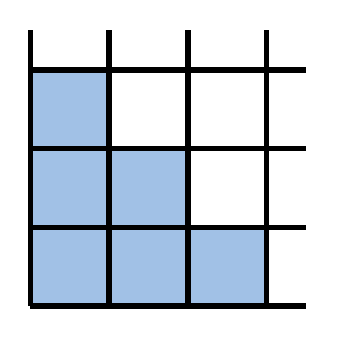
\begin{tikzpicture}[]
\fill[fill=rvwvcq,opacity=0.4] (0,0) -- (0,3) -- (1,3) -- (1,2) -- (2,2) -- (2,1) -- (3,1) -- (3,0) -- cycle;
\draw [line width=2pt,color=black] (-0,-0) grid (3.5,3.5);
\end{tikzpicture}
\end{figure*}

无限大的方格纸上有一些棋子, 每个格子最多有一个棋子, 可以按下面的规则操作: 如果一个棋子的上邻和右邻的格子内都没有棋子, 可以去掉这个棋子, 并在上邻和右邻各放一个棋子. 纸上有 6 个特殊标记的格子, 下面的给出两种开局情况, 问是否能通过有限次操作让这 6 个被标记的方格内都没有棋子:

(a) 整个纸上只有这 6 个被标记的格子中有棋子;

(b) 整个纸上只有左下角被标记的那一个格子内有棋子.

~

解: 给每个格子一个数值, 其中左下角被标记的格子值是 1, 其他格子的值是它左边或下边数值的一半. 
\begin{figure*}[htbp]
\centering
\definecolor{rvwvcq}{rgb}{0.08235294117647059,0.396078431372549,0.7529411764705882}
\begin{tikzpicture}[evaluate={
		int \i, \j;
		for \i in {0,...,4}{
			for \j in {0,...,4}{
				\a{\i,\j} = int((2^(\i+\j)));
			};
		};
	}]
\fill[fill=rvwvcq,opacity=0.4] (0,0) -- (0,3) -- (1,3) -- (1,2) -- (2,2) -- (2,1) -- (3,1) -- (3,0) -- cycle;
\fill[fill=red!30] (0,3) -- (0,5.5) -- (1,5.5) -- (1,3) -- cycle;
\fill[fill=orange!30] (3,0) -- (5.5,0) -- (5.5,1) -- (3,1) -- cycle;
\draw [line width=2pt,color=black] (-0,-0) grid (5.5,5.5);
\foreach \x in {0,...,4}
	\foreach \y in {0,...,4}
		\node at (\x+0.5,\y+0.5) {$\frac{1}{\a{\x,\y}}$};
\end{tikzpicture}
\end{figure*}

当去掉一个棋子时, 会在右边和上边相邻的位置加入一个棋子, 操作前后棋子的数值之和不变. 所有格子的数值之和为
\begin{align*} 
S &= \left(1+\frac{1}{2} + \frac{1}{4} + \cdots \right) + \left(\frac{1}{2} + \frac{1}{4} + \frac{1}{8} + \cdots \right) + \cdots \\
	&= \left( 1+\frac{1}{2} + \frac{1}{4} + \cdots \right) \left( 1+\frac{1}{2} + \frac{1}{4} + \cdots \right) \\
%	&= 2\cdot 2 \\
	&= 4.
\end{align*}

被标记部分的数值之和为 $ 11/4 $, 其余部分数值为 $ 5/4 $, 因为每个格子上最多只能有一个棋子, 所以 (a) 是不可能达到的.

对于 (b) 问题, 初始只有左下角有一个棋子, 不管怎么变, 最左一列和最下一行有且只有一个棋子. 腾空被标记区域后, 这两部分的数值之和最大是 $ 1/4 $, 而剩下白色区域的数值之和是 $ 3/4 $, 如果要达到初始时的数值, 必须白色区域所有格子上都有棋子, 这在有限次操作内是不可能实现的.


\newpage
%------------------------------------------------------------------------------%
\noindent 环球城市数学竞赛~ 1982 春季~ 初中组

设 $\{a_k\}$ 是两两不同, 且每项均大于 1 的无穷整数列. 求证: 在 $\{a_k\}$ 中可以找到无穷多项, 使得 $a_k > k$.

~

思路: 考虑 $a_1$ 的值, 例如假设 $a_1 = 5$, 再看 $a_1, a_2, a_3, a_4, a_5$ 这几个数, 由鸽笼原理, 它们不可能都小于 $5$, 总要有一个数大于 $5$, 找到其中最大的数, 例如是 $a_3=7$, 然后再看 $a_1, \cdots, a_7$, 它们不可能都小于 $7$, 至少有一个会大于 $7$, 再找这 7 个数中的最大值, 例如是 $a_7 = 10$, 这样可以一直构造下去.

~

证明: 可以用归纳构造一个无穷严格递增的正整数序列 $k_1, k_2, \cdots$, 使得对于任意正整数 $n$, 有 $a_{k_n} > k_n$, 且若正整数 $i < k_n$, 则 $a_i < a_{k_n}$.

事实上, $n=1$时, 因为 $a_1 > 1$, 只要取 $k_1 = 1$ 即可. 假设 $k_n$ 已经选好, 因为 $2, 3, \cdots, a_{k_n}$ 是 $a_{k_n} - 1$ 个数, 而 $a_1, a_2, \cdots, a_{a_{k_n}}$ 有 $a_{k_n}$ 个不同的数, 所以它们中至少有一个数大于 $a_{k_n}$. 取 $a_{k_{n+1}} = \max\{a_1, a_2, \cdots, a_{a_{k_n}}\}$, 则 $a_{k_{n+1}} > a_{k_n}$. 而下标 $k_{n+1}$ 是满足 $1 \le k_{n+1} \le a_{k_n}$ 的, 所以有 $a_{k_{n+1}} > a_{k_n} \ge k_{n+1}$. 又因为 $a_{k_{n+1}}$ 是 $a_1, a_2, \cdots, a_{a_{k_n}}$ 中的最大值, 所以当 $i < k_{n+1}$ 时, $a_i < a_{k_{n+1}}$. 

另一方面, 由归纳假设, 当$1\le i \le k_n$ 时,  $a_i \le a_{k_n}$, 但是 $a_{k_{n+1}} > a_{k_n}$, 所以必然有 $k_{n+1} > k_n$, 这就说明了 $k_n$ 是严格单调递增的. 从而存在无穷多个 $k_n$ 满足 $a_{k_n} > k_n$.

\newpage
%------------------------------------------------------------------------------%
\noindent 关于国际象棋棋盘的智力题

~

\noindent 问题:

有一个 $ 8\times 8$ 的网格, 按从左到右从上到下的顺序依次编号 $0, 1, \cdots, 63 $, 再给每个格子涂上黑色或白色, 使得每行每列恰有 $ 4 $ 个白色和 $ 4 $ 个黑色格子. 求证: 白色格子的编号之和等于黑色格子编号之和.

~

\noindent 证明:

只要按八进制写出编号, 第一行格子编号是 $00, 01, \cdots, 07 $, 第二行是 $ 10, 11, \cdots, 17 $ 等等.
因为每行每列恰有 $ 4 $ 个白色格子, 取出所有白色编号, 恰有 $ 4 $ 个低位是 $ 0 $, 恰有 $ 4 $ 个低位是 $ 1 $, 等等, 并且恰有 $ 4 $ 个高位是 $ 0 $, 恰有 $ 4 $ 个高位是 $ 1 $, 等等. 黑色编号也如此, 所以二者的和相等. 

~

\noindent 问题: 

用 $ 32 $ 个 $ 1\times 2 $ 的多米诺骨牌覆盖 $ 8 \times 8 $ 的棋盘, 证明: 无论怎样覆盖, 使用的横的和竖的骨牌数量一定都是偶数个.

~

\noindent 证明:

不失一般性, 逐行考虑每行竖的骨牌个数. 因为每个横的牌能覆盖两个格子, 所以第一行竖的骨牌个数一定是偶数个. 将第一行的这些竖的骨牌拿掉, 这可能会造成第二行有一些 (偶数个) 空隙, 所以第二行剩余的竖的骨牌也是偶数个. 再拿掉第二行剩余的竖的骨牌, 考虑第三行剩余的竖的骨牌, 等等. 这样每一行都拿掉了偶数个竖的骨牌, 到第 $ 8 $ 行时全部拿掉 (其实第 $ 7 $ 行拿掉后就已经没有了). 所以竖的骨牌个数是偶数个. 横的骨牌也是同理.

~

\noindent 问题:

$8\times 8$的标准国际象棋棋盘上任意挖掉一个黑格和一个白格, 证明: 剩下的部分仍然可以用 $ 31 $ 个 $ 1\times 2 $ 的多米诺骨牌完全覆盖.

~

\noindent 证明: 

可以画一条环路经过原棋盘的所有格子, 而不重复, 例如下图就是一种方案.
\begin{figure*}[htbp]
\centering
\begin{tikzpicture}[scale=0.5]
\draw[shift={+(1,1)}] (0,0) -- (0,8) -- (8,8) -- (8,0) -- cycle;
\foreach \x in {2,4,6,8}
	\foreach \y in {2,4,6,8}
		\draw[fill=gray!50] (\x,\y) rectangle ++(1,1);
\foreach \x in {1,3,5,7}
	\foreach \y in {1,3,5,7}
		\draw[fill=gray!50] (\x,\y) rectangle ++(1,1);
\draw [line width=1pt,dashed,shift={+(1,1)}] (0.5,0.5) -- (0.5,7.5) -- (7.5,7.5) -- (7.5,0.5) -- (6.5,0.5) -- (6.5,6.5) -- (5.5,6.5) -- (5.5,0.5) -- (4.5,0.5) -- (4.5,6.5) -- (3.5,6.5) -- (3.5,0.5) -- (2.5,0.5) -- (2.5,6.5) -- (1.5,6.5) -- (1.5,0.5) -- cycle;
\draw[pattern=crosshatch, pattern color=black] (2,5) rectangle ++(1,1);
\draw[pattern=crosshatch, pattern color=black] (5,3) rectangle ++(1,1);
\end{tikzpicture}
\end{figure*}

环路上总是黑白格子交替出现, 任意删掉一黑一白两个格子, 环路被分成两段, 每段路径仍然是一黑一白交替出现, 因此只要用骨牌分别沿着每段路径铺垫, 就可以覆盖剩余的棋盘.


\newpage
%------------------------------------------------------------------------------%
\noindent 来自"Heard on the street"

\noindent 问题: You are given a set of scales and 12 marbles. The scales are of the old balance variety. That is, a small dish hangs from each end of a rod that is balanced in the middle. The device enables you to conclude either that the contents of the dishes weigh the same or that the dish that falls lower has heavier contents than the other.

The 12 marbles appear to be identical. In fact, 11 of them are identical, and one is of a different weight. Your task is to identify the unusual marble and discard it. You are allowed to use the scales three times if you wish, but no more.

Note that the unusual marble may be heavier than the others, or it may be lighter. You are asked to both identify it and determine whether it is heavy or light.

大意: 有 12 个外观一样的石头, 其中 11 个重量是一样的, 剩下的那个可能偏轻或者偏重. 给一个天平, 要用最多 3 次称量找出异常的石头, 以及判断它是偏轻还是偏重. 

~ 

\noindent 解:

把石头编号为 1-12. 用 $ n^+ $ 和 $ n^- $ 表示第 $ n $ 号石头偏重和偏轻的情况, 这样共有 $ 12\times 2 = 24 $ 种可能的异常情况. 我们希望把这些异常情况分成相等的几份, 每次称量筛选出一份, 这样即使在最坏情况下后续的候选情况不至于太多. 

先举一个例子. 显然需要在天平两边放相同数量的石头才有意义. 如果第一次称天平左右两边放 1 号和 2 号. 结果可能有 3 种, 每一种对应的异常情况如下:
\begin{figure*}[htbp]
\centering
\setlength\extrarowheight{2pt}
\begin{tabular}{l|l|l}
\hline
Case 1 & 偏左  & $1^+, 2^-$ \\ \hline
Case 2 & 偏右  & $1^-, 2^+$ \\ \hline
Case 3 & 平衡  & $3^+, 3^-, 4^+, 4^-, 5^+, 5^-, 6^+, 6^-, \cdots, 12^+, 12^- $ \\ \hline
\end{tabular}
\end{figure*}

如果恰好天平平衡了, 需要用 2 次称量分辨 20 种异常情况, 是做不到的. 此外, 经过上表可以观察到, 如果天平偏向某一侧, 则说明这一侧的某个石头可能偏重, 或者对侧的某个石头偏轻. 如果天平平衡说明异常的石头不在天平上. 

我们往两边放更多的石头, 各放 4 个的时候异常情况可以被均分. 例如, 1-4在左边, 5-8在右边, 得到下表:
\begin{figure*}[htbp]
\centering
\setlength\extrarowheight{2pt}
\begin{tabular}{l|l|l}
\hline
Case 1 & 偏左  & $1^+, 2^+, 3^+, 4^+, 5^-, 6^-, 7^-, 8^- $ \\ \hline
Case 2 & 偏右  & $1^-, 2^-, 3^-, 4^-, 5^+, 6^+, 7^+, 8^+ $ \\ \hline
Case 3 & 平衡  & $9^+, 9^-, 10^+, 10^-, 11^+, 11^-, 12^+, 12^- $ \\ \hline
\end{tabular}
\end{figure*}

Case 1 和 Case 2 筛选出来的情况是对称的, 我们选其中偏左的这个结果 (Case 1) 来分析第二次称量的策略. 经过一些尝试, 可以左边放 $\{1,5,9\}$, 右边放 $\{2,3,6\}$. 注意此时如果天平偏左, 说明有 $ \{ 1^+, 5^+, 9^+, 2^-, 3^-, 6^- \}$ 这些可能, 再结合第一次称量的结论, 就只剩下 $ \{1^+, 6^- \} $. 类似的推出偏右和平衡的情况. 最后, 有下表的分析:
\begin{figure*}[htbp]
\centering
\setlength\extrarowheight{2pt}
\begin{tabular}{l|l|l}
\hline
Case 1.1 & 偏左  & $1^+, 6^-$ \\ \hline
Case 1.2 & 偏右  & $2^+, 3^+, 5^- $ \\ \hline
Case 1.3 & 平衡  & $4^+, 7^-, 8^- $ \\ \hline
\end{tabular}
\end{figure*}

对于 Case 1.1, 只要再比较 1 号和 2 号; 平衡对应 $ 6^- $; 偏向 1 号对应 $ 1^+ $, 不会出现偏向 2 号的情况. 

对于 Case 1.2, 比较 2 号和 3 号, 偏向哪个说明哪个是异常, 且偏重; 平衡说明是 $ 5^- $. 

对于 Case 1.3, 比较 7 号和 8 号, 偏向哪个说明另一边是异常, 且更轻; 平衡说明是 $ 4^+ $.

Case 2 和 Case 1是类似的. 

再看 Case 3, 经过一些尝试, 可以左边放 $ \{ 1,9 \} $, 右边放 $ \{ 10, 11 \} $, 得到下表:
\begin{figure*}[htbp]
\centering
\setlength\extrarowheight{2pt}
\begin{tabular}{l|l|l}
\hline
Case 3.1 & 偏左  & $9^+, 10^-, 11^-$ \\ \hline
Case 3.2 & 偏右  & $9^-, 10^+, 11^+ $ \\ \hline
Case 3.3 & 平衡  & $12^+, 12^- $ \\ \hline
\end{tabular}
\end{figure*}

Case 3.1 和 Case 1.3 类似, 而 Case 3.2 和 Case 1.2 类似. 

对于 Case 3.3, 只要比较 1 号和 12 号, 就可知道 12 号是偏轻还是偏重, 同样这里不存在平衡的情况.

~

Heard on the Street 后面之后又提出了一个更复杂的拓展问题: 石头数量变成 90 个, 其中仍然有一个质量与其他的不同, 问至少需要称多少次能在最坏情况下找出, 以及具体方法.

如果仍然向上面那样, 后续的策略要依赖于前面的称量结果进行调整, 就需要逐个情况分析验证, 工作量巨大. 这里借鉴纠错码的思路给出一个通用的解法, 每一步称量策略不依赖于前面的结果.

回到 12 个石头的问题. 我们将称量这一操作用数学的语言描述. 设编号 $ i $ 的石头质量为 $ m_i $, 取值为 $ \{-1,0,1\} $, 分别对应偏轻, 正常, 偏重的情况. 天平的倾斜状态同样可以定义为 $ \{-1, 0, 1\} $, 对应偏左,平衡,偏右的情况, 于是, 每个左盘的石头贡献了负的力矩, 右盘的石头贡献正的力矩. 当然, 对于质量是 $-1$ 的石头则是反过来. 将每个石头放在左盘还是右盘用 $ w_i $ 表示, 同样 $w_i$ 的取值范围是 $ \{-1, 0, 1\} $. 于是, 天平状态 $ r $ 可以表示成:
\[ r = \sum_{i=1}^N{w_im_i} = \boldsymbol{w}^T\boldsymbol{m} .\]

也就是两个向量 $ \boldsymbol{w} $ 和 $ \boldsymbol{m} $ 的内积.
这里把 $ \boldsymbol{m} $ 向量称为质量向量, 每次称质量向量都是固定不变的, $ \boldsymbol{w} $ 向量和 $ r $ 可能会变. 此外, $ \boldsymbol{m} $ 向量有 11 个元素为 0, 剩下那个元素可能是 $\pm{1}$.

记三次称量使用的 $ \boldsymbol{w} $ 向量分别是 $ \boldsymbol{w}_1 $, $ \boldsymbol{w}_2 $, $ \boldsymbol{w}_3 $, 它们构成了一个 $ 3\times 12 $ 的矩阵 $ \mathbf{W} $, 称为称量矩阵. 三次称量的天平状态构成了一个 3 维列向量, 称为结果向量. 我们的目标是确定矩阵 $ \mathbf{W} $ 的具体形式, 使得根据结果向量可以推出质量向量的非零元是哪个, 以及值是多少. 

注意到每次称量左右两边的石头个数要一样才有意义, 说明 $ \mathbf{W} $ 每一行 $+1$ 和 $-1$ 个数要相等.

继续观察, 假设第 $ j $ 个石头异常且偏重, 则质量向量第 $ j $ 个元素是 $ 1 $, 其余是 $0$, 与称量矩阵相乘后, 结果向量正好是称量矩阵的第 $ j $ 列. 如果是第 $ j $ 个石头偏轻, 则结果向量是负的矩阵第 $ j $列. 一旦定下来称量矩阵, 它乘以不同质量向量得出的结果向量一定不能相同. 而质量向量有 24 种可能性, 对应的结果向量就是称量矩阵的每一列以及负的每一列. 换言之, 称量矩阵每一列和负的每一列向量构成的集合必须两两不相等, 否则就会有不同的质量向量得出相同的结果矩阵, 这是没法确定具体是哪个质量矩阵.

到目前为止, 已经找到了确定称量矩阵的 3 个条件:
\begin{enumerate}
\item 任意两列不同
\item 任意两列和不为零向量
\item 每行元素之和为 0
\end{enumerate}

下面进行构造. 先写出所有由 $ \{-1,0,1\} $ 组成的 3 维列向量, 共 27 个, 除掉零向量, 还剩 26 个. 将它们分成 13 组, 每组互为相反向量. 每组最多选一个向量作为称量矩阵的一列, 这样就自动满足前两个条件. 至于第三个条件, 需要做一些搜索. 总的来说, 这个问题是 NP-Hard 的. 搜索的原则是, 每一行的 $-1, 0, 1$ 三个数要尽量一样多. 如果前 $ k $ 行已经满足条件, 在不改变前 $ k $ 行之和的前提下调整后面的行. 直到全部满足条件.

这里构造一个称量矩阵:
\begin{figure*}[htbp]
\centering
\setlength\extrarowheight{2pt}
\begin{tabular}{|l|l|l|l|l|l|l|l|l|l|l|l|}
\hline
-1 & -1 & -1 & -1 &  1 &  1 &  1 &  1 &  0 &  0 &  0 &  0\\
 1 &  1 & -1 & -1 &  1 &  0 &  0 &  0 & -1 & -1 &  1 &  0\\
-1 &  0 &  1 & -1 &  0 & -1 &  1 &  0 &  1 & -1 &  0 &  1 \\
\hline
\end{tabular}
\end{figure*}

如何根据结果向量找到异常的石头以及判断轻重呢? 每次称量矩阵的一行放置石头, -1 表示对应的石头在左边, 1 表示对应的石头在右边, 0 表示不参与此次称量. 我们得到了结果向量, 拿它跟称量矩阵每一列比较, 如果第 $ j $ 列等于结果向量, 说明第 $ j $ 个石头偏重; 如果是第 $ j $的相反向量等于结果向量, 说明第 $ j $ 个石头偏轻. 


~

\noindent Heard on the Street 给出的拓展问题的三个解法, 也在此记录.

\noindent 解法1: 

将石头分成 3 个组, 每组 30 个, 记为 $ A, B, C $. 先称 $A$ 和 $B$.

Case 1: 平衡. 再把 $C$ 分成 $ 10\times 3 $ 的三组: $C.A, C.B, C.C$, 比较 $C.A$ 和 $C.B$.

Case 1.1: 再次平衡. 异常石头在剩下的 $C.C$ 里, 只要再加入 2 个正常的石头, 套用 12 个石头的解法, 再称 3 次就行.

Case 1.2: $C.A < C.B$. 将存疑的这两个组的石头分别再分成 $ 3+4+3 $ 的 3 份出来. 同样还是以后缀 $ A,B,C $ 表示三个小组, 例如 $C.A.A$ 和 $C.A.C$ 有 3 个石头, $ C.A.B $有 4 个. 取 $ C.A.A + C.B.B $ 和 $ C.A.B + C.B.A $ 比较.

Case 1.2.1: $ C.A.A + C.B.B = C.A.B + C.B.A $, 说明是 $ C.A.C < C.B.C $, 再将存疑的两组各取一个比较.

Case 1.2.1.1: $ C.A.C.A + C.B.C.A = C.A.C.B + C.B.C.B $, 说明是 $ C.A.C.C < C.B.C.C $, 只要拿 $ C.A.C.C $ 与任何一个正常的石头比较就行.

Case 1.2.1.2: $ C.A.C.A + C.B.C.A < C.A.C.B + C.B.C.B $, 说明是 $ C.A.C.A < C.B.C.B $, 跟 Case 1.2.1.1 类似.

Case 1.2.1.3: $ C.A.C.A + C.B.C.A > C.A.C.B + C.B.C.B $, 说明是 $ C.A.C.B < C.B.C.A $, 也跟 Case 1.2.1.1 类似.

Case 1.2.2: $ C.A.A + C.B.B < C.A.B + C.B.A $, 说明 $ C.A.A < C.B.A $, 存疑的两组各有 3 个石头, 跟 Case 1.2.1 一样.

Case 1.2.3: $ C.A.A + C.B.B > C.A.B + C.B.A $, 说明 $ C.A.B < C.B.B $, 存疑的两组各有 4 个石头, 并且知道要么是 $ C.A.B $ 的 4 个更轻, 要么是 $ C.B.B $ 的 4 个更重, 这跟 12 石头的问题种第一次称量不平衡的情况是一样的. 

Case 2: $A$ 和 $B$ 不平衡. 不妨设 $A < B$. 再次将 $ A $ 和 $ B $ 分别分成三组, 记为 $A.A, A.B, A.C, B.A, B.B, B.C $, 取 $ A.A $ 和 $ B.A $ 放左侧, $ A.B $ 和 $B.B $ 放右侧.

Case 2.1: $ A.A + B.A = A.B + B.B $. 说明 $ A.C < B.C $, 这与 Case 1.2 一样.

Case 2.2: $ A.A + B.A < A.B + B.B $, 说明 $ A.A < B.B $, 也跟 Case 1.2 一样.

Case 2.3: $ A.A + B.A > A.B + B.B $, 说明 $ A.B < B.A $, 还是跟 Case 1.2 一样.

Case 3: $ A > B $, 跟 Case 2 是对称的.

~

\noindent 解法2:

首先说明一个结论: 如果事先知道异常的石头是偏轻还是偏重, 那么我们可以用 $k$ 次称量, 就可以从 $3^k$ 个石头中找到异常的那个.

将 90 个石头分成 $ 90 = 81 + 9 $ 的两部分. 再将 81 的那部分分成 3 组 $ A,B,C$ , 每组 27 个. 先用两次称量, 比如 $A$ 对 $B$ 以及 $A$ 对 $C$, 可以知道这三组里哪一组有异常石头, 并且知道异常石头偏轻还是偏重. 然后用 3 次称量在 27 个候选里找到异常石头. 总共需要称 5 次.

当然也有可能是 $ A, B, C $ 全相等, 就说明异常石头在 9 的那部分里. 可以拿 9 个正常石头和它们比较, 确定异常石头偏轻还是偏重, 然后用两次称量找到异常石头; 或者在 9 个异常候选者里加入 3 个正常石头凑成 12 个石头的问题, 不管用哪种方式, 也都需要 5 次称量.

~

\noindent 解法3:

这个方法可以解更强的 120 个石头的问题, 或者更一般的 $N = \dfrac{3^n - 3}{2}$ 个石头的问题. 缺点是只能解这些特定个数的问题, 不能处理任意个数. 下面讨论 120 个石头的问题.

将 120 个石头分成 $ 40\times 3 $ 的三组, 每组内部分成 $ 1 + 3 + 9 + 27 $ 的四部分. 记为 $ \{\{1\}_A, \{3\}_A, \{9\}_A, \{27\}_A \} $, 和 $ \{\{1\}_B, \{3\}_B, \{9\}_B, \{27\}_B \} $, 以及 $ \{\{1\}_C, \{3\}_C, \{9\}_C, \{27\}_C \} $. 先比较 $A$和 $B$ 两个大组.

Case 1: $ A = B $. 异常石头在 $ C $ 组中, 此时拿 $ \{27\}_A $ 和 $ \{27\}_C $ 比. 

Case 1.1: 不平衡. 可以知道异常石头在 $ \{27\}_C $ 中, 且知道偏轻还是偏重, 需要再称 3 次找出来.

Case 1.2: 平衡. 此时再拿 $ \{9\}_A $ 和 $ \{9\}_C $ 比, 不平衡则需要再称两次, 平衡则又拿 $ \{3\}_A $ 和 $ \{1\}_C $, 等等. 不管何种情况, 总数都是 5 次.

Case 2: $ A < B $. 我们把 27 的那部分在 3 组里做一个置换, $A\leftarrow B\leftarrow C\leftarrow A$, 比较 $ \{\{1\}_A, \{3\}_A, \{9\}_A, \{27\}_B \} $ 和 $ \{\{1\}_B, \{3\}_B, \{9\}_B, \{27\}_C \} $, 剩下 $ \{\{1\}_C, \{3\}_C, \{9\}_C, \{27\}_A \} $.

Case 2.1: $\{1\}_A + \{3\}_A + \{9\}_A + \{27\}_B = \{1\}_B + \{3\}_B + \{9\}_B + \{27\}_C $. 说明异常石头在 $\{27\}_A$ 里, 且偏轻, 用 3 次称量可以找出.

Case 2.2: $\{1\}_A + \{3\}_A + \{9\}_A + \{27\}_B > \{1\}_B + \{3\}_B + \{9\}_B + \{27\}_C $. 说明异常石头在 $\{27\}_B$ 里, 且偏重, 同样用 3 次称量可以找出.

Case 2.3: $\{1\}_A + \{3\}_A + \{9\}_A + \{27\}_B < \{1\}_B + \{3\}_B + \{9\}_B + \{27\}_C $. 说明三组的 27 个石头的那部分都是正常的, 将它们丢掉, 把 9 的那部分在 3 组里做置换, 也就是比较 $ \{\{1\}_A, \{3\}_A, \{9\}_B \} $ 和 $ \{\{1\}_B, \{3\}_B, \{9\}_C \} $, 这又回到了规模更小的 Case 2. 递归下去也都需要 5 次得到结论.

Case 3: $ A > B $, 跟 Case 2 是对称的.


\newpage
%------------------------------------------------------------------------------%
\noindent 来自每日数学打卡

对于非负整数 $n$ 定义以下三种变换, 变换 $ A: n \rightarrow \lfloor\dfrac{n}{3}\rfloor$, 其中 $\lfloor x\rfloor$ 表示不超过 $x$ 的最大整数, 变换 $B: n \rightarrow 9n+1$, 变换 $C: n \rightarrow 9n+2$. 现在从 $0$ 开始, 每次随机进行变换 A, B, C, 这个过程中可能出现任意大的数, 也可能出现重复的数. 经过充分多次的变换之后, 过程中出现的数中, 不超过 15000 的不同正整数最多有多少个.

~

解: 考虑用三进制表示变换操作, 对于一个三进制数 $x$, 变换$A$相当于去掉末位数, 变换$B$相当于在末位后添加$01$, 变换$C$相当于在末位后添加$02$.

于是, 变换过程出现的数的三进制数字串满足条件 "任意两个非零数字中间至少有一个0", 或者说 "不存在连续的两个非零的数字". 另一方面, 任意满足上面条件的数都可以通过反复进行这三种变换得到. 

符合上述条件的最大的 9 位三进制数为 $(202020202)_3 = 14762 < 15000 $, 而最小的 10 位三进制数为 $3^9=
19683 > 15000$, 所以只要求不超过 9 位的满足上面条件的三进制正整数个数.

可以在 9 个位置上任选 1 到 5 个位置不相邻的位置, 每个位置填 1 或 2, 其余填 0. $n$ 个位置选 $k$ 个不相邻的位置的方法数为 $C_{n+1-k}^{k}$, (想象 $n$ 个空位, 放 $k$ 个白球, $n-k$个黑球, 要求白球之间不相邻, 则把每个白球右边绑一个黑球, 最后一个白球不绑, 算下来只有$n-k+1$个自由移动的个体, 在其中选出$k$ 个作为白球的位置, 它与白球不相邻的排列方式是一一对应的). 总计数为:
\[ 2C_9^1 + 2^2 C_8^2 + 2^3 C_7^3 + 2^4 C_6^4 + 2^5 C_5^5 = 682 .\]

\newpage
%------------------------------------------------------------------------------%

\noindent 中科大强基题

有五个矩形 $A_1, A_2, A_3, A_4, A_5$, 他们的边都是平行于直角坐标系的坐标轴(轴对齐). 求证: 一定能从其中找到这样的两个矩形, 例如 $A_4, A_5$, 使得这两个矩形的并集包含其余三个矩形的交集, 即: $(A_1\cap A2\cap A3) \subset (A_4\cup A_5)$. 

~

\noindent 思路:

考虑五个矩形的相交区域 $S$, 如果$S$不是空集, 存在至少一个点, 它的 $x$ 坐标大于所有矩形的左边界, 而小于所有矩形的右边界, $y$ 坐标大于所有矩形的下边界而小于所有矩形的上边界. 若 $S$ 是空集, 则说明存在一个矩形的左边界大于另一个矩形的右边界, 或者一个矩形的下边界大于另一个矩形的上边界的情况, 也就是说明存在两个矩形不相交. 将他们作为 $A_1, A_2$, 再随便配一个作为 $A_3$, 得到三个矩形的交为空集, 于是总是被另外两个矩形的并集所包含. 

如果 $S$ 不是空集, 考虑 $S$ 四个边界的构成. 如果来源于三个不同的矩形, 说明这三个矩形的交集就是$S$, 又因为 $S$ 是所有五个矩形的交集, 自然也被剩下两个矩形包含, 命题得证. 如果来源于更少的三角形, 也是类似. 但如果 $S$ 的边界来源于四个不同的矩形, 则这四个边界分别是原来五个矩形的左边界的最大值, 右边界的最小值, 下边界的最大值, 和上边界的最小值, 如下图所示.
\begin{figure*}[htbp]
\centering
\definecolor{rvwvcq}{rgb}{0.08235294117647059,0.396078431372549,0.7529411764705882}
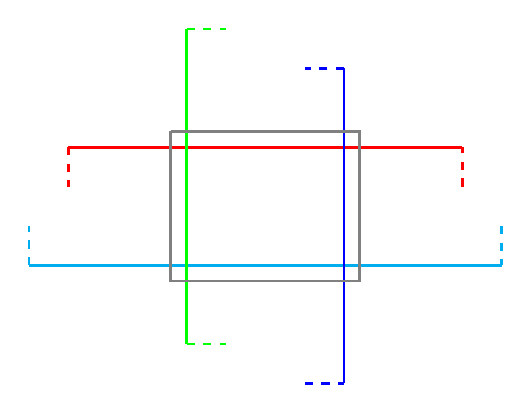
\begin{tikzpicture}[scale=1]
\draw [line width=1pt,color=red] (-2.5,1.5)-- (2.5,1.5);
\draw [line width=1pt,dash pattern=on 3pt off 3pt,color=red] (-2.5,1.5)-- (-2.5,1.0);
\draw [line width=1pt,dash pattern=on 3pt off 3pt,color=red] (2.5,1.0)-- (2.5,1.5);
\draw [line width=1pt,color=cyan] (-3,0)-- (3,0);
\draw [line width=1pt,dash pattern=on 3pt off 3pt,color=cyan] (-3,0)-- (-3,0.5);
\draw [line width=1pt,dash pattern=on 3pt off 3pt,color=cyan] (3,0.5)-- (3,0);
\draw [line width=1pt,color=green] (-1,3)-- (-1,-1);
\draw [line width=1pt,dash pattern=on 3pt off 3pt,color=green] (-1,3)-- (-0.5,3);
\draw [line width=1pt,dash pattern=on 3pt off 3pt,color=green] (-1,-1)-- (-0.5,-1);
\draw [line width=1pt,color=blue] (1,2.5)-- (1,-1.5);
\draw [line width=1pt,dash pattern=on 3pt off 3pt,color=blue] (1,2.5)-- (0.5,2.5);
\draw [line width=1pt,dash pattern=on 3pt off 3pt,color=blue] (0.5,-1.5)-- (1,-1.5);
\draw [line width=1pt,color=gray] (-1.2,1.7)-- (1.2,1.7) -- (1.2, -0.2)-- (-1.2, -0.2) -- (-1.2,1.7);
%\draw [line width=1pt,color=red] (-1.5,2)-- (-1.5,-1.2);
%\draw [line width=1pt,dash pattern=on 3pt off 3pt,color=red] (-1.5,2)-- (-1.3,2);
%\draw [line width=1pt,dash pattern=on 3pt off 3pt,color=red] (-1.3,-1.2)-- (-1.5,-1.2);
\end{tikzpicture}
\end{figure*}

考虑剩余的那个矩形$X$, 它要包含这个相交区域, 我们从 $S$ 的四个边界往外走, 如果有一个方向, 不妨假设往左走, $X$ 排在第三或更靠后, , 那么可以选择构成 $S$ 左边界的矩形与 $X$ 构成 $A_4, A_5$, 剩下三个矩形相交的部分上,下,右三个方向边界与 $S$ 一样, 左边界被推到了排第二的地方, 相比于 $S$ 多出来的那部分也被 $X$ 完全覆盖. 

反之, 如果四个方向往外走, $X$ 都是排在第二的位置, 那么我们选 $X$ 和任意两个矩形作为 $A_1, A_2, A_3$, 例如选构成 $S$上下边界的矩形. 这样三个矩形的相交区域具有上下两个方向的最"靠内"值, 左右两个方向有第二"靠内"值. 而 $A_4, A_5$ 的并集在左右两个方向至少包含了第三"靠内"的范围, 而上下两个方向也是至少包含第三靠内的范围. 所以这种情况也得证.

~ 

\noindent 严谨的证明

设每个矩形的上下左右边界对应的 $xy$ 值为 $(u_i, d_i, l_i, r_i)$. 若 $A_1 \cap A_2 = \varnothing$, 则以下 4 式至少有一个成立:
\begin{align*}
l_1 &> r_2, \\
r_1 &< l_2, \\
d_1 &> u_2, \\
u_1 &< d_2.
\end{align*}
若 $A_1\cap A_2 \neq \varnothing$, 则上述 4 式全不成立. 即有:
\begin{align*}
l_1 &< r_2, \\
l_2 &< r_1, \\
d_1 &< u_2, \\
d_2 &< u_1.
\end{align*}
为表述方便, 取等号即两边正好重合先不讨论.

同时显然存在以下关系:
\begin{align*}
l_i &< r_i, \\
d_i &< u_i.
\end{align*}
进一步可得, 若 $A_i\cap A_k\neq\varnothing,\ i,k\in\{1,2,3,4,5\}$, 则 $l_k < r_i, d_k < u_i$, 即:当任意两个矩形相交非空时, 所有矩形的"左边"在所有矩形的"右边"之左, 所有矩形的"上边"在所有矩形的"下边"之上.
可以反证, 若上述结论不成立, 譬如 $A_1$ 的"左边"在 $A_2$ 的"右边"之右, 则 $A_1$ 与 $A_2$ 的相交为空, 这与"任意两个矩形相交非空"矛盾.

若两个矩形 $A_1, A_2$ (或其他两个矩形) 相交非空, 其交集也是边平行于坐标轴的矩形, 记作 $B_{12}$, 它的"上边"为 $\min(u_1, u_2)$, "下边"为 $\max(d_1, d_2)$, "左边"为 $\max(l_1,l_2)$, "右边"为 $\min(r_1, r_2)$. 反之, 若矩形四边满足上述条件, 则该矩形必为 $A_1, A_2$ 的交集. 3个, 4个或5个矩形的交集同理.

下面分情况讨论.

1. 若存在两个矩形区域不相交 (交集为空), 譬如 $A_1\cap A_2=\varnothing$, 则 $(A_1\cap A_2\cap A_3)=\varnothing$, 而空集是任意非空集合的子集, 即 $ \varnothing\subset(A_4\cup A_5) $, 于是当存在两个不相交的矩形时, $(A_1\cap A_2\cap A_3) \subset (A_4\cup A_5)$ 成立. 


2. 若不存在两个相交为空的矩形, 即5个矩形中任意两个矩形相交都非空, 由前述结论, 记5个矩形的交集为 $B_{12345}$, 其"上边"为 $\min\{u_i\}$, "下边"为 $\max\{d_i\}$, "左边"为 $\max\{l_i\}$, "右边"为 $\min\{r_i\}$. 

2.1 若 $B_{12345}$ 的各边同属于5个矩形中的一个, 两个, 或三个, 譬如 $A_1, A_2, A_3$, 设 $B_{12345}$ 的上下左右边的$xy$值为 $u,d,l,r$, 此时显然有:
\begin{align*}
u &= \min(u_1, u_2, u_3), \\
d &= \max(d_1, d_2, d_3), \\
l &= \max(l_1, l_2, l_3), \\
r &= \min(r_1, r_2, r_3).
\end{align*}
即 $B_{12345} = (A_1\cap A_2\cap A_3)$, 而 $B_{12345}$ 是全部5个矩形的交集, 所以必为 $A_4, A_5$ 的子集. 故此时 $(A_1\cap A_2\cap A_3) \subset (A_4\cup A_5)$ 成立. 

2.2 若 $B_{12345}$ 的四边分别属于四个不同的矩形, 不妨设为 $A_1, A_2, A_3, A_4$, 如下图, 根据抽屉原理, 必有 $A_5$ 的四边不在 $B_{12345}$ 的四边之列.

2.2.1 假设 $A_5$ 的4条边正好在 $B_{12345}$ 的次外圈, 即 $A_5$ 只与 $u_1, r_2, d_3, l_4$ 相交.
\begin{figure*}[htbp]
\centering
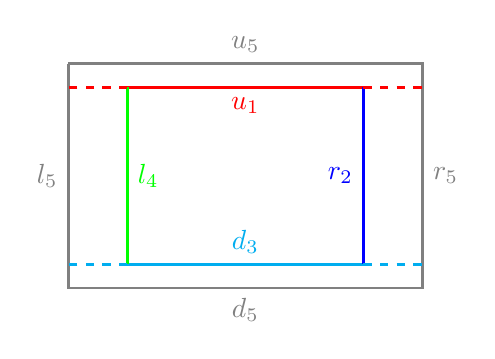
\begin{tikzpicture}[scale=1.5]
\draw [line width=1pt,color=red] (-1,1.5)-- node[below] {$u_1$} (1,1.5) ;
\draw [line width=1pt,color=cyan] (-1,0)-- node[above] {$d_3$} (1,0);
\draw [line width=1pt,color=green] (-1,1.5)-- node[right] {$l_4$} (-1,0);
\draw [line width=1pt,color=blue] (1,1.5)-- node[left] {$r_2$} (1,0);
\draw [line width=1pt,color=gray] (-1.5,1.7)--  node[above] {$u_5$} (1.5,1.7) -- node[right] {$r_5$} (1.5, -0.2) -- node[below] {$d_5$}(-1.5, -0.2) -- node[left] {$l_5$}(-1.5,1.7);
\draw [line width=1pt,dash pattern=on 3pt off 3pt,color=red] (-1,1.5)-- (-1.5,1.5);
\draw [line width=1pt,dash pattern=on 3pt off 3pt,color=cyan] (-1,0)-- (-1.5,0);
\draw [line width=1pt,dash pattern=on 3pt off 3pt,color=red] (1,1.5)-- (1.5,1.5);
\draw [line width=1pt,dash pattern=on 3pt off 3pt,color=cyan] (1,0)-- (1.5,0);
\end{tikzpicture}
\end{figure*}

显然, 
\begin{align*}
u_1 &= \min(u_1, u_3, u_5), \\
d_3 &= \max(d_1, d_3, d_5), \\
l_5 &= \max(l_1, l_3, l_5), \\
r_5 &= \min(r_1, r_3, r_5).
\end{align*}
由 $u_1, d_3, l_5, r_5$ 围成的矩形等于 $(A_1\cap A_3\cap A_5)$, 记作 $B_{135}$, 其中 $B(u_1, d_3, l_5, l_4)$ 部分, 因为 $l_5 > l_2, l_4 < r_2$, 该区域为 $A_2$ 的子集. 同理 $B(u_1, d_3, r_2, r_5)$ 部分, 因为 $r_2>l_4, r_5<r_4$, 该区域为 $A_4$ 的子集. 又因为中间部分 $B_{12345}$ 是5个矩形任意一个的子集, 所以有: $(A_1\cap A_3\cap A_5) \subset (A_2\cup A_4)$. 

2.2.2 若 $B_{12345}$ 的次外圈并不全是 $A_5$ 的四边, 譬如下图 $u_2$ 紧挨着处于 $u_1$ 之上.
\begin{figure*}[htbp]
\centering
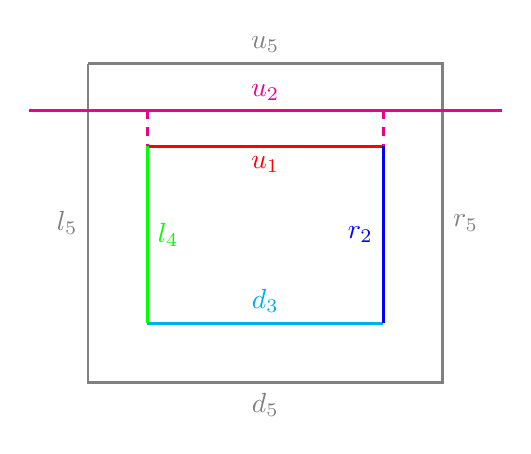
\begin{tikzpicture}[scale=1.5]
\draw [line width=1pt,color=red] (-1,1.5)-- node[below] {$u_1$} (1,1.5) ;
\draw [line width=1pt,color=cyan] (-1,0)-- node[above] {$d_3$} (1,0);
\draw [line width=1pt,color=green] (-1,1.5)-- node[right] {$l_4$} (-1,0);
\draw [line width=1pt,color=blue] (1,1.5)-- node[left] {$r_2$} (1,0);
\draw [line width=1pt,color=gray] (-1.5,2.2)--  node[above] {$u_5$} (1.5,2.2) -- node[right] {$r_5$} (1.5, -0.5) -- node[below] {$d_5$}(-1.5, -0.5) -- node[left] {$l_5$}(-1.5,2.2);
\draw [line width=1pt,color=magenta] (-2,1.8)-- node[above] {$u_2$} (2,1.8);
\draw [line width=1pt,dash pattern=on 3pt off 3pt,color=magenta] (-1,1.8)-- (-1,1.5);
\draw [line width=1pt,dash pattern=on 3pt off 3pt,color=magenta] (1,1.8)-- (1,1.5);
\end{tikzpicture}
\end{figure*}

\noindent 此时, 
\begin{align*}
u_2 &= \min(u_2, u_3, u_4), \\
d_3 &= \max(d_2, d_3, d_4), \\
l_4 &= \max(l_2, l_3, l_4), \\
r_2 &= \min(r_2, r_3, r_4).
\end{align*}
即 $B(u_2, d_3, l_4, r_2) = (A_2\cap A_3\cap A_4)$. 由图可知 $B(u_2, d_3, l_4, r_2)\subset A_5$, 即有 $(A_2\cap A_3\cap A_4) \subset (A_1\cup A_5)$.

当矩形两边重合而不重叠时, 视为相交为空集. 按照情况1处理, 或视为相交为宽度为0的特殊矩形, 按情况2处理.

综上, 原式得证.

\newpage
%------------------------------------------------------------------------------%
\noindent 来自网络

乒乓球队集训进行单打循环赛, 甲乙丙三人参加, 第一轮两人先打, 第三人轮空, 胜者下轮继续, 败者下场换人, 如此循环. 比赛结束后, 甲乙丙各打了15, 10, 17场, 问谁输了第二场比赛.

~

解: 三人总共打了 42 场, 所以有 21 场对局. 乙轮空了 11 场, 而一个人不会连续轮空两场. 所以只能是奇数的 11 场是乙在轮空, 意味着第二场比赛乙输了, 所以才在第三场轮空.








































